\section{Wavelet Trees} \label{sec:wavelet_trees}

Building upon the concepts established for bitvectors in Section~\ref{sec:bitvectors}, we now extend our focus to sequences over general alphabets using \emph{Wavelet Trees}. Introduced by Grossi, Gupta, and Vitter \cite{GrossiWT2003}, the wavelet tree is a highly versatile data structure. It functions as a self-index, capable of representing a sequence $S[1..n]$ drawn from an alphabet $\Sigma = \{1, \dots, \sigma\}$ within space close to its compressed size, while supporting fundamental query operations directly on this representation and allowing reconstruction of the original sequence data. This characteristic makes wavelet trees a cornerstone in applications like compressed full-text indexing, for example within the FM-index \cite{ferragina2000opportunistic}, where they provide efficient support for the essential \textsf{rank} queries during the backward search phase \cite{WTForALL}.

While the core idea of hierarchical alphabet partitioning shares conceptual similarities with earlier structures, such as Chazelle's structure for geometric point grids \cite{Chazelle1988} and Kärkkäinen's work on repetition-based indexing \cite{karkkainen1999repetition}, the specific formulation and operational capabilities defined by Grossi et al. \cite{GrossiWT2003} established the wavelet tree as a broadly applicable tool for sequence processing \cite{WTForALL}. Its flexibility derives from its capacity to represent data variously as sequences, permutations, or point grids \cite{WTForALL, WTFromTheoryToPractice, TheMyriadVirtuesWT}.

We consider a sequence $S[1..n] = s_1s_2\dots s_n$, with $s_i \in \Sigma = \{1, \dots, \sigma\}$. The primary operations of interest are generalizations of those defined for bitvectors:
\begin{itemize}
    \item \texttt{Access(S, i)}: $S \times [1..n] \to \Sigma$. Returns the symbol $S[i]$.
    \item \textsf{rank}$_c(S, i)$: $S \times \Sigma \times [0..n] \to [0..n]$. Returns the number of occurrences of symbol $c$ in the prefix $S[1..i]$, i.e., $|\{j \mid 1 \le j \le i, S[j]=c\}|$. We define $\textsf{rank}_c(S, 0) = 0$.
    \item \textsf{select}$_c(S, j)$: $S \times \Sigma \times [1..n] \to [1..n] \cup \{\perp\}$. Returns the position (index) $k$ such that $S[k]=c$ and $\textsf{rank}_c(S, k) = j$. If the $j$-th occurrence does not exist, it returns a special symbol $\perp$.
\end{itemize}
A naive approach using $\sigma$ distinct bitvectors $B_c$ (where $B_c[i]=1$ if and only if $S[i]=c$) reduces these operations to bitvector rank/select ($\textsf{rank}_c(S,i) = \textsf{rank}_1(B_c,i)$ and $\textsf{select}_c(S,j) = \textsf{select}_1(B_c,j)$). However, augmenting these bitvectors for $O(1)$ time queries using the methods of Section~\ref{sec:bitvectors} requires $n\sigma + o(n\sigma)$ total bits, which is inefficient compared to the $n \lceil \log \sigma \rceil$ bits of the plain representation, especially for large $\sigma$ \cite{navarro2016compact}. Wavelet trees offer a significantly more space-conscious solution.

\subsection{Structure and construction}

The standard wavelet tree for a sequence $S[1..n]$ over $\Sigma = \{1, \dots, \sigma\}$ is a balanced binary tree structure. Each node $v$ corresponds to an alphabet sub-range $[a_v, b_v] \subseteq \Sigma$ and implicitly represents the subsequence $S_v$ containing all characters $s_i$ from the original sequence $S$ such that $s_i \in [a_v, b_v]$, maintaining their relative order.

The construction proceeds recursively:
\begin{itemize}
    \item The root node $v_{root}$ corresponds to the full alphabet range $[1, \sigma]$ and the entire sequence $S_{v_{root}} = S$.
    \item For an internal node $v$ representing the range $[a_v, b_v]$ with $a_v < b_v$:
          \begin{enumerate}
              \item Define a midpoint $m_v = \lfloor (a_v + b_v) / 2 \rfloor$.
              \item Store a bitmap $B_v[1..|S_v|]$ where $B_v[k] = 0$ if the $k$-th character of $S_v$ is in $[a_v, m_v]$, and $B_v[k] = 1$ if it is in $[m_v+1, b_v]$.
              \item Recursively construct the left child $v_l$ for the alphabet range $[a_v, m_v]$ and the subsequence $S_{v_l}$ formed by characters $s \in S_v$ with $s \le m_v$.
              \item Recursively construct the right child $v_r$ for the alphabet range $[m_v+1, b_v]$ and the subsequence $S_{v_r}$ formed by characters $s \in S_v$ with $s > m_v$.
          \end{enumerate}
    \item A leaf node $v$ represents a single symbol alphabet range $[a_v, a_v]$ (i.e., $a_v=b_v$) and stores no bitmap.
\end{itemize}
The height of this tree is $h = \lceil \log \sigma \rceil$. The construction process, detailed in Algorithm~\ref{alg:build_wt}, takes $O(n \log \sigma)$ time, as each symbol from $S$ is processed at each level of the tree.

\begin{algorithm}[ht!]
    \caption{Building a wavelet tree}\label{alg:build_wt}
    % ... (Algorithm code remains the same as provided) ...
    \begin{algorithmic}
        % ... (Algorithm code remains the same as provided) ...
        \Function{build\_wt}{$S,n$}
        \State $T \gets build(S,n,1,\sigma)$
        \State \Return $T$
        \EndFunction
        \Function {build}{$S,n,a,b$} \Comment{\small{Takes a string $S[1,n]$ over $[a,b]$}}
        \If {$a = b$}
        \State Free S
        \State \Return null
        \EndIf
        \State $v \gets$ new node
        \State $m \gets \lfloor (a+b)/2 \rfloor$
        \State $z \gets 0$ \Comment{\small{number of elements in $S$ that are $\leq m$}}
        \For {$i \gets 1$ to $n$}
        \If {$S[i] \leq m$}
        \State $z \gets z+1$
        \EndIf
        \EndFor

        \State Allocate strings $S_{left}[1,z]$ and $S_{right}[1,n-z]$
        \State Allocate bitmap $v.B[1,n]$
        \State $z \gets 0$

        \For {$i \gets 1$ to $n$}
        \If {$S[i] \leq m$}
        \State \texttt{bitclear}($v.B,i$) \Comment{\small{set $i$-th bit of $v.B$ to 0}}
        \State $z \gets z+1$
        \State $S_{left}[z] \gets S[i]$
        \Else
        \State \texttt{bitset}($v.B,i$) \Comment{\small{set $i$-th bit of $v.B$ to 1}}
        \State $S_{right}[i-z] \gets S[i]$
        \EndIf
        \EndFor

        \State Free S
        \State $v.left \gets \texttt{build}(S_{left},z,a,m)$
        \State $v.right \gets \texttt{build}(S_{right},n-z,m+1,b)$
        \State Pre-process $v.B$ for $rank$ and $select$ queries
        \State \Return $v$
        \EndFunction
    \end{algorithmic}
\end{algorithm}

The space usage of this pointer-based wavelet tree consists of the bitmaps and the pointers. The bitmaps across all nodes at any given level collectively store exactly $n$ bits. With $h = \lceil \log \sigma \rceil$ levels, the total space for bitmaps is $n \lceil \log \sigma \rceil$. The tree has $\sigma$ leaves and $\sigma-1$ internal nodes. Storing child and parent pointers (e.g., $3(\sigma-1)$ pointers, each $\approx \log \sigma$ bits) adds an overhead of $O(\sigma \log \sigma)$ bits (or $O(\sigma \log n)$ if indices into an array are used), which can dominate for large $\sigma$. Each bitmap $B_v$ must also be augmented with $o(|S_v|)$ bits to support constant-time rank/select (Section~\ref{sec:bitvectors}), contributing an additional $o(n \log \sigma)$ bits overall.

\begin{figure}[h]
    % ... (Tikz code remains the same as provided) ...
    \centering
    % \tikzstyle{every node}=[font=\footnotesize]
    % \begin{tikzpicture}[
    %         scale=0.5,
    %         level distance=4.5cm,
    %         level 1/.style={sibling distance=12.3cm},
    %         level 2/.style={sibling distance=6.3cm},
    %         level 3/.style={sibling distance=3cm},
    %         level 4/.style={sibling distance=1.6cm},
    %         level 5/.style={sibling distance=0.7cm},
    %         level 6/.style={sibling distance=0.7cm},
    %         level 7/.style={sibling distance=0.7cm}]  % Added level 7 style
    %     \node[align=center] {\texttt{wookies\_wield\_wicked\_weapons\_with\_wisdom\$}\\\texttt{111100101001001001000100111101010010}}
    %     child {node[align=center] {\texttt{ie\_ied\_iced\_ea\_ih\_id\$}\\\texttt{110111010110100110110}}
    %             child {node[align=center] {\texttt{\_\_c\_a\_\_\&}\\\texttt{00101000}}
    %                     child {node[align=center] {\texttt{\_\_\_\_\_\$}\\\texttt{000001}}
    %                             child {node[align=center] {\texttt{\$}} edge from parent node[left] {0}}  % Added level 7 node
    %                             child {node[align=center] {\texttt{\_}} edge from parent node[right] {1}}  % Added level 7 node
    %                             edge from parent node[left] {0}}
    %                     child {node[align=center] {\texttt{ca}\\\texttt{10}}
    %                             child {node[align=center] {\texttt{a}} edge from parent node[left] {0}}  % Added level 7 node
    %                             child {node[align=center] {\texttt{c}} edge from parent node[right] {1}}  % Added level 7 node
    %                             edge from parent node[right] {1}}
    %                     edge from parent node[left] {0}}
    %             child {node[align=center] {\texttt{ieiediedeihid}\\\texttt{1010010001110}}
    %                     child {node[align=center] {\texttt{iiiihi}\\\texttt{111101}}
    %                             child {node[align=center] {\texttt{h}} edge from parent node[left] {0}}  % Added level 7 node
    %                             child {node[align=center] {\texttt{i}} edge from parent node[right] {1}}  % Added level 7 node
    %                             edge from parent node[left] {0}}
    %                     child {node[align=center] {\texttt{eededed}\\\texttt{1101010}}
    %                             child {node[align=center] {\texttt{d}} edge from parent node[left] {0}}  % Added level 7 node
    %                             child {node[align=center] {\texttt{e}} edge from parent node[right] {1}}  % Added level 7 node
    %                             edge from parent node[right] {1}}
    %                     edge from parent node[right] {1}}
    %             edge from parent node[left] {0}}
    %     child {node[align=center] {\texttt{wookswlwkwponswtwsom}\\\texttt{11101101011101111110}}
    %             child {node[align=center] {\texttt{klknm}\\\texttt{00011}}
    %                     child {node[align=center] {\texttt{klk}\\\texttt{010}}
    %                             child {node[align=center] {\texttt{k}} edge from parent node[left] {0}}  % Added level 7 node
    %                             child {node[align=center] {\texttt{l}} edge from parent node[right] {1}}  % Added level 7 node
    %                             edge from parent node[left] {0}}
    %                     child {node[align=center] {\texttt{nm}\\\texttt{10}}
    %                             child {node[align=center] {\texttt{m}} edge from parent node[left] {0}}  % Added level 7 node
    %                             child {node[align=center] {\texttt{n}} edge from parent node[right] {1}}  % Added level 7 node
    %                             edge from parent node[right] {1}}
    %                     edge from parent node[left] {0}}
    %             child {node[align=center] {\texttt{wooswwwposwtwso}\\\texttt{100111100111110}}
    %                     child {node[align=center] {\texttt{oopoo}\\\texttt{00100}}
    %                             child {node[align=center] {\texttt{o}} edge from parent node[left] {0}}  % Added level 7 node
    %                             child {node[align=center] {\texttt{p}} edge from parent node[right] {1}}  % Added level 7 node
    %                             edge from parent node[left] {0}}
    %                     child {node[align=center] {\texttt{swwwswtws}\\\texttt{1011101110}}
    %                             child {node[align=center] {\texttt{s}}}
    %                             child {node[align=center] {\texttt{wwwwtw}\\\texttt{111101}}
    %                                     child {node[align=center] {\texttt{t}} edge from parent node[left] {0}}  % Added level 7 node
    %                                     child {node[align=center] {\texttt{w}} edge from parent node[right] {1}}  % Added level 7 node
    %                                     edge from parent node[right] {1}}
    %                             edge from parent node[right] {1}}
    %                     edge from parent node[right] {1}}
    %             edge from parent node[right] {1}};
    % \end{tikzpicture}
    \includegraphics[width=\textwidth]{assets/WT_full.pdf}
    \caption{\small Wavelet tree for the sequence \texttt{wookies\_wield\_\dots}} \label{fig:wavelet_tree_example}
\end{figure}

\subsubsection*{Tracking symbols}
The wavelet tree supports the primary sequence operations by translating them into traversals involving bitvector rank/select queries.

\subsubsection{Access}
Computing $\textsf{access}(S, i)$ involves a top-down traversal from the root $v_{root}$. At each internal node $v$ (representing range $[a_v, b_v]$ with midpoint $m_v$), we examine the bit $B_v[i_v]$, where $i_v$ is the current index within the node's implicit sequence $S_v$. If $B_v[i_v] = 0$, we proceed to the left child $v_l$ (range $[a_v, m_v]$) and update the index to $i_{v_l} = \textsf{rank}_0(B_v, i_v)$. If $B_v[i_v] = 1$, we proceed to the right child $v_r$ (range $[m_v+1, b_v]$) and update the index to $i_{v_r} = \textsf{rank}_1(B_v, i_v)$. This repeats until a leaf node representing a single symbol $[a, a]$ is reached; this $a$ is $S[i]$. The process performs $\lceil \log \sigma \rceil$ bitvector \textsf{rank} operations in $O(\log \sigma)$ time. Algorithm~\ref{alg:access_wt} details this.

\begin{algorithm}[h!]
    \caption{\textsf{Access} queries on a wavelet tree}\label{alg:access_wt}
    \small
    \begin{algorithmic}
        \Function {access}{$T,i$} \Comment{\small{$T$ is the sequence $S$ seen as a wavelet tree}}
        \State $v \gets T_{root}$ \Comment{\small{start at the root node}}
        \State $[a,b] \gets [1,\sigma]$
        \While{$a \neq b$}
        \If{$access(v.B,i) =0$} \Comment{\small{$i$-th bit of the bitmap of $v$}}
        \State $i \gets rank_0(v.B,i)$
        \State $v \gets v.left$ \Comment{\small{move to the left child of node $v$}}
        \State $b \gets \lfloor (a+b)/2 \rfloor$
        \Else
        \State $i \gets rank_1(v.B,i)$
        \State $v \gets v.right$ \Comment{\small{move to the right child of node $v$}}
        \State $a \gets \lfloor (a+b)/2 \rfloor +1$
        \EndIf
        \EndWhile
        \State \Return $a$
        \EndFunction
    \end{algorithmic}
\end{algorithm}

\subsubsection{Select}
Computing $\textsf{select}_c(S, j)$ involves an upward traversal from the leaf node $u$ corresponding to symbol $c$. Let the index within the leaf level be $j_u = j$. To move to the parent $v$, we determine if $u$ is the left ($v_l$) or right ($v_r$) child. If $u = v_l$, the corresponding index in the parent's bitmap $B_v$ is $j_v = \textsf{select}_0(B_v, j_u)$. If $u = v_r$, the index is $j_v = \textsf{select}_1(B_v, j_u)$. We repeat this process, updating $j$ at each level, until the root node is reached. The final index $j_{root}$ is the position of the $j$-th $c$ in $S$. This requires $\lceil \log \sigma \rceil$ bitvector \textsf{select} operations in $O(\log \sigma)$ time. Algorithm~\ref{alg:select_wt} shows the recursive structure.

\begin{algorithm}
    \caption{\texttt{Select} queries on a wavelet tree}\label{alg:select_wt}
    \small
    \begin{algorithmic}
        \Function{$\textsf{select}_c$}{$S,j$}
        \State \Return $\textsf{select}(T._{root},1, \sigma, c, j)$
        \EndFunction


        \Function{$\textsf{select}$}{$v,a,b,c,j$}
        \If{$a = b$}
        \State \Return $j$
        \EndIf
        \If {$c \leq \lfloor (a+b)/2 \rfloor$}
        \State $j$ $\gets$ $\textsf{select}(v.left, a, \lfloor (a+b)/2 \rfloor, c, j)$
        \Return $select_0(v.B,j)$
        \Else
        \State $j$ $\gets$ $\textsf{select}(v.right, \lfloor (a+b)/2 \rfloor +1, b, c, j)$
        \State \Return $select_1(v.B,j)$
        \EndIf
        \EndFunction
    \end{algorithmic}
\end{algorithm}

\subsubsection{Rank}
Computing $\textsf{rank}_c(S, i)$ uses a top-down traversal similar to \textsf{access}. We start at the root $v_{root}$ with index $i_{root} = i$. At each node $v$ (range $[a_v, b_v]$, midpoint $m_v$), we check if the target symbol $c$ belongs to the left sub-range ($c \le m_v$) or the right sub-range ($c > m_v$). If $c \le m_v$, we descend to the left child $v_l$ and update the index to $i_{v_l} = \textsf{rank}_0(B_v, i_v)$. If $c > m_v$, we descend to the right child $v_r$ and update the index to $i_{v_r} = \textsf{rank}_1(B_v, i_v)$. The traversal continues until the leaf node $u$ corresponding to symbol $c$ is reached. The final index $i_u$ at this leaf is the value $\textsf{rank}_c(S, i)$. This requires $\lceil \log \sigma \rceil$ bitvector \textsf{rank} operations in $O(\log \sigma)$ time. Algorithm~\ref{alg:rank_wt} formalizes this.

\begin{example}
    Consider the computation of $\textsf{rank}_e(S, 13)$ shown in \autoref{fig:rank_example_wt}. We start at the root with index $i=13$. Here, \emph{e} corresponds to bit 0, so we compute $\textsf{rank}_0(13) = 6$ and descend left with the new index $i=6$. At this node, \emph{e} corresponds to bit 1; evaluating $\textsf{rank}_1(6) = 5$, we proceed right with index $i=5$. In the next node, \emph{e} maps to bit 0; calculating $\textsf{rank}_0(5) = 3$, we descend left with $i=3$. We reach the node for \emph{e}, where it corresponds locally to bit 1. The final computation is $\textsf{rank}_1(3) = 2$. Thus, $\textsf{rank}_e(S, 13) = 2$.
\end{example}


\begin{figure}[h]
    \centering
    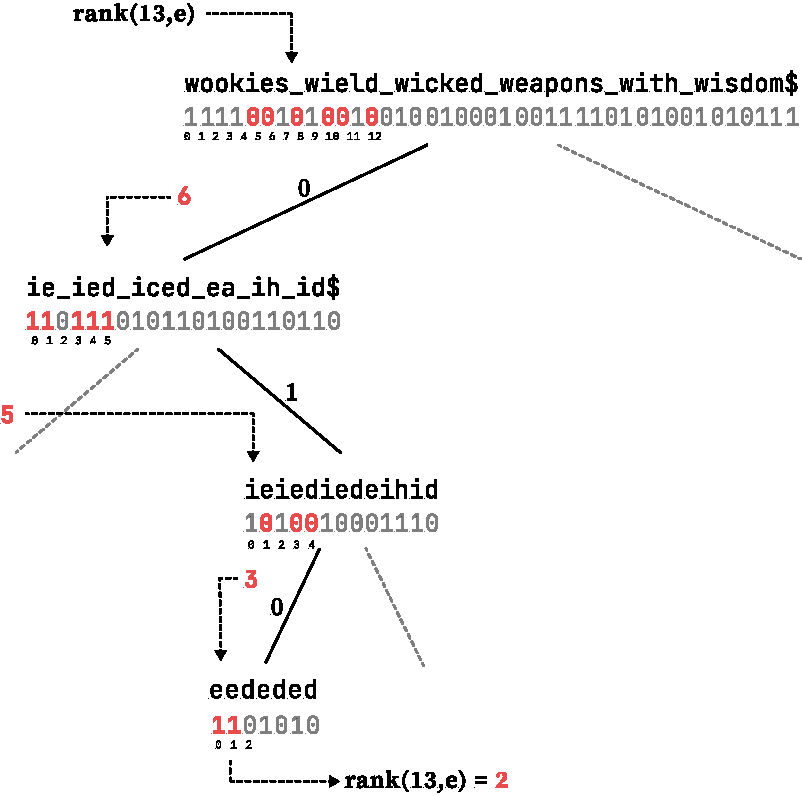
\includegraphics[width=0.9\textwidth]{assets/WT_rank_example.pdf}
    \caption{\textsf{rank}$_e(S,13)$ on the wavelet tree of \autoref{fig:wavelet_tree_example}.}
    \label{fig:rank_example_wt}
\end{figure}


\begin{algorithm}[h!]
    \caption{\texttt{Rank} queries on a wavelet tree}\label{alg:rank_wt}
    % ... (Algorithm code remains the same as provided) ...
    \begin{algorithmic}
        \Function{$\textsf{rank}_c$}{$S,i$}
        \State $v \gets T_{root}$ \Comment{\small{start at the root node}}
        \State $[a,b] \gets [1,\sigma]$
        \While {$a \neq b$}
        \If {$c \leq \lfloor (a+b)/2 \rfloor$}
        \State $i \gets rank_0(v.B,i)$
        \State $v \gets v.left$ \Comment{\small{move to the left child of node $v$}}
        \State $b \gets \lfloor (a+b)/2 \rfloor$
        \Else
        \State $i \gets rank_1(v.B,i)$
        \State $v \gets v.right$ \Comment{\small{move to the right child of node $v$}}
        \State $a \gets \lfloor (a+b)/2 \rfloor +1$
        \EndIf
        \EndWhile
        \State \Return $i$
        \EndFunction
    \end{algorithmic}
\end{algorithm}

\emph{Pointerless Representation}: To remove the $O(\sigma \log \sigma)$ pointer overhead, the pointerless wavelet tree concatenates bitmaps level-wise \cite{MAKINEN2007332, MAKINEN2006703}. Let $B_l$ be the concatenated bitmap for level $l$. If a node $v$ at level $l$ corresponds to the range $[s_v, e_v]$ in $B_l$, its left child's range in $B_{l+1}$ is
\[
    [(l+1)n + \textsf{rank}_0(B_l, s_v-1) + 1, (l+1)n + \textsf{rank}_0(B_l, e_v)]
\]
Its right child's range is
\[
    [(l+1)n + z_l + \textsf{rank}_1(B_l, s_v-1) + 1, (l+1)n + z_l + \textsf{rank}_1(B_l, e_v)]
\]
where $z_l = \textsf{rank}_0(B_l, n)$ is the total $0$-count at level $l$. This achieves $n \lceil \log \sigma \rceil + o(n \log \sigma)$ total space. Navigation requires extra \textsf{rank} operations per level compared to the pointer-based version (\cite{claude2015wavelet}), which can impact practical performance, although the asymptotic query time remains $O(\log \sigma)$.

\subsection{Compressed Wavelet Trees} \label{sec:compressed_WT}

The standard wavelet tree representations (pointer-based and pointerless) achieve space proportional to $n \log \sigma$. However, when the sequence $S$ itself is compressible (i.e., its empirical entropy is lower than $\log \sigma$), it is desirable for the index structure to reflect this compressibility. Wavelet trees can be adapted to achieve space bounds related to the empirical entropy of $S$, primarily through two main strategies: directly compressing the bitmaps stored within the nodes, or reshaping the tree based on symbol frequencies.

\subsubsection{Compressing the Bitvectors} \label{subsec:compressing_bitvectors}

This approach maintains the balanced binary structure of the wavelet tree but replaces the plain bitmaps $B_v$ at each internal node $v$ with compressed representations that still support efficient \textsf{rank} and \textsf{select} queries. As explored in Section~\ref{subsec:elias_fano_compression}, various techniques exist for compressing sparse or biased bitvectors. If we employ a representation for each $B_v$ (of length $N_v = |S_v|$) that uses $N_v \mathcal{H}_0(B_v) + o(N_v)$ bits while maintaining $O(1)$ query times for \textsf{rank} and \textsf{select} (e.g., using structures based on Raman et al. \cite{RRR2002} or improved variants \cite{patrascu2008succincter}), the total space complexity aggregates advantageously.

\begin{theorem}[Entropy-Compressed WT Space (Bitmaps) \cite{GrossiWT2003, navarro2016compact, ferragina2007compressed}] \label{thm:h0_bitmap_wt_space}
    A wavelet tree for $S[1..n]$ over $\Sigma=\{1,\dots,\sigma\}$, using node bitmaps compressed to their zero-order entropy with $O(1)$-time rank/select support, can be stored in
    \[ n \mathcal{H}_0(S) + o(n \log \sigma) \text{ bits}. \]
    The query times for \textsf{access}, \textsf{rank}, and \textsf{select} remain $O(\log \sigma)$.
\end{theorem}
\begin{proof}[Proof sketch]
    The core idea relies on the property that the sum of zero-order entropies of the bitmaps at any level $l$ is upper bounded by the sum at level $l-1$. Summing across all internal nodes, the total space for the compressed bitmaps relates directly to the zero-order entropy of the original sequence $S$:
    \[\sum_{v \text{ internal}} |S_v| \mathcal{H}_0(B_v) = n \mathcal{H}_0(S)\]
    The $o(n \log \sigma)$ term arises from aggregating the sublinear $o(N_v)$ overheads from each node's rank/select structure across all levels. Since rank/select on each compressed bitmap is $O(1)$, the total query time remains determined by the tree height, $O(\log \sigma)$.
\end{proof}

While theoretically achieving optimal space relative to $H_0(S)$, practical implementations using compressed bitmaps (like those based on RRR found in libraries such as SDSL \cite{gog2014theory}) can exhibit higher query latency compared to using plain, uncompressed bitmaps due to the computational overhead of performing rank/select on the compressed format \cite{claude2015wavelet}.

\subsubsection{Huffman-Shaped Wavelet Trees} \label{subsec:huffman_shaped_wavelet_trees}

Instead of compressing the content (bitmaps), this strategy compresses the structure itself by adapting the tree shape to the symbol frequencies $f_c = \textsf{rank}_c(S, n)$ in $S$. The wavelet tree is given the shape of a Huffman tree \cite{huffman1952method} constructed for the symbols based on their frequencies \cite{grossi2004indexing, makinen2004new}. In this structure, a symbol $c$ occurring $f_c$ times resides at a leaf at depth $|h(c)|$, where $h(c)$ is its Huffman code. The bitmaps $B_v$ are stored uncompressed at the internal nodes.

The total number of bits stored in the plain bitmaps across the entire tree is precisely the length of the Huffman-encoded sequence:
\[ \sum_{c \in \Sigma} f_c |h(c)| \quad \le \quad n(\mathcal{H}_0(S)+1) \text{ bits}. \]
Adding the overhead for rank/select support on these plain bitmaps ($o(n(\mathcal{H}_0(S)+1))$ total) and the space to store the Huffman model itself (e.g., $O(\sigma \log \sigma)$ bits, reducible for canonical codes \cite{claude2015wavelet}), gives the total space.

\begin{theorem}[Huffman-Shaped WT Performance \cite{makinen2004new, navarro2016compact}] \label{thm:huffman_wt_space_time}
    A Huffman-shaped wavelet tree using plain bitmaps (with $O(1)$ rank/select support) occupies space bounded by
    \[ n(\mathcal{H}_0(S)+1) + o(n(\mathcal{H}_0(S)+1)) + O(\sigma \log \sigma) \text{ bits}. \]
    It supports \textsf{access}, \textsf{rank}, and \textsf{select}. The worst-case query time is $O(d_{max})$, where $d_{max}$ is the maximum depth (potentially $O(n)$, but typically bounded to $O(\log \sigma)$ \cite{navarro2007compressed}). The average query time, assuming queries are distributed according to symbol frequencies ($f_c/n$), is $O(1+\mathcal{H}_0(S))$.
\end{theorem}

This approach achieves compression related to $\mathcal{H}_0(S)$ through structural adaptation rather than bitmap compression, often leading to faster average query times ($O(1+\mathcal{H}_0(S))$ vs $O(\log \sigma)$) for statistically skewed query distributions, while using potentially simpler and faster plain bitmap rank/select structures. Pointerless versions based on canonical Huffman codes are also possible \cite{claude2015wavelet}.

\subsubsection{Higher-Order Entropy Compression} \label{subsec:higher_order_entropy}

To capture statistical dependencies beyond symbol frequencies, wavelet trees are often used on the Burrows-Wheeler Transformed \cite{burrows1994block} sequence $S^{\textsc{Bwt}}$. The \textsc{Bwt} groups symbols preceded by the same context of length $k$, making $S^{\textsc{Bwt}}$ highly compressible by methods sensitive to local statistics. The $k$-th order empirical entropy, $H_k(S)$, quantifies this context-dependent compressibility (see Section~\ref{sec:higher_order_entropy}). It is known that $\sum_{A \in \Sigma^k} |S_A| \mathcal{H}_0(S_A) = n \mathcal{H}_k(S)$, where $S_A$ is the sequence of symbols following context $A$ \cite{manzini2001analysis}.

Building a single wavelet tree over the entire $S^{\textsc{Bwt}}$ and using zero-order entropy compression on its internal bitmaps (as in Section~\ref{subsec:compressing_bitvectors}) allows the structure to achieve space related to $H_k(S)$ for the original sequence $S$.

\begin{theorem}[$H_k$-Compressed WT \cite{navarro2007compressed, TheMyriadVirtuesWT}] \label{thm:hk_wt_space}
    Let $S^{\textsc{Bwt}}$ be the Burrows-Wheeler Transform of $S$. A wavelet tree built over $S^{\textsc{Bwt}}$ using node bitmaps compressed to their zero-order entropy (requiring $N_v \mathcal{H}_0(B_v) + o(N_v)$ bits per node $v$) occupies a total space of
    \[ n \mathcal{H}_k(S) + o(n \log \sigma) \text{ bits} \]
    for any $k \le \alpha \log_\sigma n$ ($0 < \alpha < 1$).
\end{theorem}
\begin{proof}[Proof sketch]
    The space bound follows because the zero-order entropy of the wavelet tree bitmaps over $S^{\textsc{Bwt}}$ sums to $n \mathcal{H}_0(S^{\textsc{Bwt}})$, and $\mathcal{H}_0(S^{\textsc{Bwt}})$ effectively captures $\mathcal{H}_k(S)$ due to the context-grouping property of the \textsc{Bwt} \cite{manzini2001analysis, navarro2007compressed}. The $o(n \log \sigma)$ term accumulates the overheads of the compressed rank/select structures.
\end{proof}

This structure supports the \textsf{rank} operations on $S^{\textsc{Bwt}}$ needed for FM-index pattern matching in $O(\log \sigma)$ time per operation.

This connection is crucial for compressed full-text indexing. Practical variants exist, such as partitioning $S^{\textsc{Bwt}}$ and using Huffman-shaped wavelet trees on the blocks \cite{karkkainen2011fixed}, which may offer different practical performance trade-offs. The choice between RLE and GE for bitmap encoding in this context was analyzed in \cite{TheMyriadVirtuesWT}, favoring RLE-like approaches for achieving $H_k$.

\subsection{Wavelet Matrices and Quad Vectors} \label{sec:wavelet_matrices_and_quad_vectors}

Further refinements address practical performance bottlenecks, primarily memory latency during tree traversal and the overhead associated with large alphabets in pointerless or Huffman representations.

\subsubsection{The Wavelet Matrix}
The wavelet matrix \cite{claude2015wavelet} provides an alternative layout for the pointerless wavelet tree that simplifies navigation and improves speed. It maintains the level-wise concatenated bitmaps $B_0, B_1, \dots, B_{h-1}$ (where $h = \lceil \log \sigma \rceil$) and stores the counts $z_l = \textsf{rank}_0(B_l, n)$ for each level $l$. The key difference lies in the mapping between levels: a position $i$ in $B_l$ corresponding to a 0-bit maps to position $\textsf{rank}_0(B_l, i)$ in $B_{l+1}$, while a position corresponding to a 1-bit maps to position $z_l + \textsf{rank}_1(B_l, i)$ in $B_{l+1}$.

\begin{theorem}[Wavelet Matrix Performance \cite{claude2015wavelet}] \label{thm:wm_perf}
    The wavelet matrix represents $S[1..n]$ using
    \[ n \lceil \log \sigma \rceil + o(n \log \sigma) \text{ bits} \]
    (where $o(n \log \sigma)$ is for rank/select support on the $h$ bitmaps, and the $z_l$ values require negligible $O(\log \sigma \log n)$ bits). It supports \textsf{access}, \textsf{rank}, and \textsf{select} queries in $O(\log \sigma)$ time, executing exactly one bitvector rank or select operation per level traversed.
\end{theorem}

This simplified navigation avoids the extra rank operations needed in the strict pointerless WT and eliminates pointer overhead, making it practically faster than pointerless trees and competitive with pointer-based trees, especially for large $\sigma$ \cite{claude2015wavelet}. It can also be combined with bitmap compression or specialized Huffman shaping \cite{claude2015wavelet}.

\subsubsection{4-ary (Quad) Wavelet Trees}
To combat the $O(\log \sigma)$ cache misses inherent in traversing a binary tree, 4-ary wavelet trees reduce the tree height to $h' = \lceil (\log \sigma)/2 \rceil$ \cite{QWT}. Each internal node partitions its alphabet range $[a_v, b_v]$ into four sub-ranges based on the next two bits in the symbols' binary representation. Instead of a bitmap, each node stores a \emph{quad vector} $Q_v$ (a sequence over $\{0, 1, 2, 3\}$ or $\{00, 01, 10, 11\}$) indicating to which of the four children each symbol belongs.

Supporting queries requires specialized rank/select operations on these quad vectors. Structures achieving $O(1)$ time for quad vector rank/select with $o(N_v \log 4) = o(N_v)$ bits of overhead per node (where $N_v$ is the quad vector length) have been developed \cite{QWT}.

\begin{theorem}[4-ary WT Performance \cite{QWT}] \label{thm:qwt_perf}
    A 4-ary wavelet tree using $O(1)$-time rank/select structures on quad vectors represents $S[1..n]$ in
    \[ n \lceil \log \sigma \rceil + o(n \log \sigma) \text{ bits} \]
    and supports \textsf{access}, \textsf{rank}, and \textsf{select} in $O(\log \sigma)$ time, specifically requiring $O(\lceil (\log \sigma)/2 \rceil)$ quad vector rank or select operations.
\end{theorem}
\begin{proof}[Proof sketch]
    Each level effectively stores 2 bits per original symbol. With $\approx (\log \sigma)/2$ levels, the total space for the quad vectors is $n \times 2 \times (\log \sigma)/2 = n \log \sigma$ bits. The $o(n \log \sigma)$ term accounts for the aggregated overhead of the quad vector rank/select structures. The query time is determined by the reduced tree height.
\end{proof}

The principal advantage lies in the potential halving of cache misses during queries, leading to significant practical speedups in latency-bound scenarios, as demonstrated experimentally in \cite{QWT}, particularly when implemented as a 4-ary wavelet matrix.
